\documentclass[11pt,a4paper]{article}
\usepackage[T1]{fontenc}
\usepackage[utf8]{inputenc}
\usepackage{lmodern}
\usepackage{textcomp}
\usepackage[left=1.8cm,right=1.8cm,top=2.3cm,bottom=2.2cm,headheight=14pt,headsep=8pt]{geometry}
\usepackage{multicol}
\usepackage{xcolor}
\usepackage{fancyhdr}
\usepackage{graphicx}
\usepackage{array}
\usepackage{amsmath,amssymb}
\usepackage{setspace}
\usepackage{longtable}
\graphicspath{{../}}
\definecolor{ygreen}{RGB}{46,139,87}
\renewcommand{\normalsize}{\fontsize{10.9}{13.4}\selectfont}
\renewcommand{\familydefault}{\rmdefault}
\setlength{\parindent}{0pt}
\setlength{\columnsep}{0.8cm}
\setlength{\columnseprule}{0.4pt}
\setlength{\multicolsep}{3pt plus 1pt minus 1pt}
\renewcommand{\textsubscript}[1]{\ensuremath{_{\text{\fontsize{8}{8}\selectfont #1}}}}
\renewcommand{\textsuperscript}[1]{\ensuremath{^{\text{\fontsize{8}{8}\selectfont #1}}}}
\newcommand{\diqqat}[1]{\par\smallskip\noindent\textbf{Diqqat!} #1\par\medskip}
\newcommand{\javob}{\par\smallskip\noindent\textbf{Javob:} \rule[-2pt]{7.5cm}{0.4pt}\par\smallskip\noindent\textbf{Diqqat!} Javobingizni javoblar varaqasiga ko`chirib yozing.\par\medskip}
\pagestyle{fancy}
\fancyhf{}
\renewcommand{\headrulewidth}{0.4pt}
\fancyhead[L]{\textit{Milliy sertifikat 2026. Kimyo}}
\fancyhead[R]{20-variant}
\fancyfoot[L]{\fontsize{8}{9}\selectfont \textcopyright{} Colba maktabi, 2026}
\fancyfoot[C]{\thepage}
\fancypagestyle{first}{\fancyhf{}\renewcommand{\headrulewidth}{0pt}\fancyfoot[L]{\fontsize{8}{9}\selectfont \textcopyright{} Colba maktabi, 2026}\fancyfoot[C]{\thepage}}
\begin{document}
\normalsize
\thispagestyle{first}
\noindent\fcolorbox{ygreen}{white}{\parbox{\dimexpr\linewidth-2\fboxsep-2\fboxrule\relax}{%
\textbf{\fontsize{13}{15}\selectfont Nazorat testi}\ \textit{\fontsize{10}{12}\selectfont $\cdot$ Aralash test $\cdot$ 20-variant}\hfill
\begin{tabular}[t]{@{}r@{}}\textit{Milliy sertifikat 2026. Kimyo}\\ \textbf{\textit{\fontsize{8}{9}\selectfont Vaqt:}} \textit{\fontsize{10}{12}\selectfont 180 daqiqa}\end{tabular}}}
\par\medskip
\noindent\textit{Davriy jadvaldan foydalanish mumkin.}
\par\medskip
\begin{multicols}{2}
\noindent\textbf{1.} 1 g He 127 \textdegree{}C va 1 atm bosimda qancha hajm (l) egallaydi? (R = 0,082 l$\cdot$atm/(mol$\cdot$K))

\noindent A)~\textsl{8,2} \hfill B)~\textsl{16,4} \hfill C)~\textsl{4,1} \hfill D)~\textsl{5,6}\par
\vspace{4pt}
\noindent\textbf{2.} Quyidagi tuzlarning qaysilari suvli eritmasi kislotali muhitga ega? 1) NH\textsubscript{4}Cl; 2) KNO\textsubscript{3}; 3) FeCl\textsubscript{3}; 4) Na\textsubscript{2}SO\textsubscript{4}

\noindent A)~\textsl{1, 3} \hfill B)~\textsl{2} \hfill C)~\textsl{1, 2} \hfill D)~\textsl{2, 3, 4}\par
\vspace{4pt}
\noindent\textbf{3.} Quyidagilarni jism va moddalarga ajrating: mixga, qaychi, etanol, alyuminiy, kislorod, osh tuzi. Ulardan nechtasi modda?

\noindent A)~\textsl{4} \hfill B)~\textsl{5} \hfill C)~\textsl{3} \hfill D)~\textsl{2}\par
\vspace{4pt}
\noindent\textbf{4.} Jadvalda bog`lar hosil qiluvchi atomlarning elektrmanfiyliklari berilgan:
\begin{center}
\renewcommand{\arraystretch}{1.15}
\begin{tabular}{|c|c|c|}\hline
\textbf{Bog`} & \textbf{EM (1-atom)} & \textbf{EM (2-atom)} \\ \hline
Na--Cl & 0,9 & 3 \\ \hline
N--H & 3 & 2,1 \\ \hline
H--F & 2,1 & 4 \\ \hline
Mg--O & 1,2 & 3,5 \\ \hline
\end{tabular}
\end{center}
Qaysi bog` eng qutbli (eng ko`p ionli xarakterga ega)?

\noindent A)~\textsl{Na--Cl} \hfill B)~\textsl{Mg--O} \hfill C)~\textsl{N--H} \hfill D)~\textsl{H--F}\par
\vspace{4pt}
\noindent\textbf{5.} 3 mol AlCl\textsubscript{3} va 2 mol HNO\textsubscript{3} suvda eritilib, eritma hajmi 5 l ga yetkazildi. Eritmadagi barcha ionlarning umumiy molyar \textbf{konsentratsiyasini (mol/l) aniqlang} (kuchli elektrolitlar to`liq dissotsilanadi).

\noindent A)~\textsl{1} \hfill B)~\textsl{3,2} \hfill C)~\textsl{6,4} \hfill D)~\textsl{1,6}\par
\vspace{4pt}
\noindent\textbf{6.} N\textsubscript{2} + 3H\textsubscript{2} $\rightleftarrows$ 2NH\textsubscript{3} reaksiyasida N\textsubscript{2} va H\textsubscript{2} stexiometrik nisbatda olingan umumiy 8 mol aralashma muvozanat qaror topganda doimiy T va \textit{V} da bosim 25\% ga kamaydi. Muvozanatdagi NH\textsubscript{3} ning \textbf{miqdorini (mol) aniqlang.}

\noindent A)~\textsl{1} \hfill B)~\textsl{3} \hfill C)~\textsl{2} \hfill D)~\textsl{4}\par
\vspace{4pt}
\noindent\textbf{7.} N\textsubscript{2} va CO\textsubscript{2} dan iborat 13,44 l (n.sh.) aralashmaning massasi 21,6 g. Aralashmadagi N\textsubscript{2} ning \textbf{massasini (g) aniqlang.}

\noindent A)~\textsl{13,2} \hfill B)~\textsl{8,4} \hfill C)~\textsl{16,8} \hfill D)~\textsl{4,2}\par
\vspace{4pt}
\noindent\textbf{8.} Mishyak atomida d-pog`onachadagi elektronlar \textbf{sonini aniqlang} (\textit{Z} = 33).

\noindent A)~\textsl{10} \hfill B)~\textsl{11} \hfill C)~\textsl{9} \hfill D)~\textsl{12}\par
\vspace{4pt}
\noindent\textbf{9.} Grafikda tuzning eruvchanligi (g/100 g suv) haroratga bog`liq ko`rsatilgan.
\begin{center}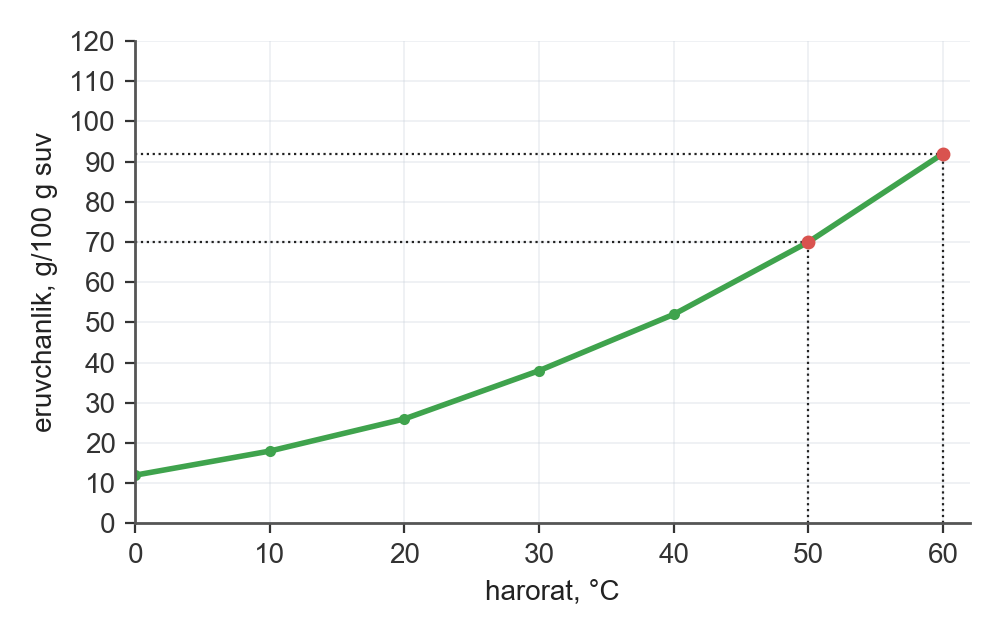
\includegraphics[width=0.86\linewidth]{rasmlar/gen/sol_v20_0.png}\end{center}
50 \textdegree{}C da to`yingan 360 g eritma 60 \textdegree{}C gacha qizdirildi. Eritmani yana to`yingan holatga keltirish uchun necha gramm tuz qo`shish kerak?

\noindent A)~\textsl{22} \hfill B)~\textsl{88} \hfill C)~\textsl{181,78} \hfill D)~\textsl{44}\par
\vspace{4pt}
\noindent\textbf{10.} Jadvalda Na\textsubscript{2}CO\textsubscript{3} ning ikki eritmasi haqida ma'lumot berilgan:
\begin{center}
\renewcommand{\arraystretch}{1.15}
\begin{tabular}{|c|c|c|}\hline
\textbf{Eritma} & \textbf{Massasi, g} & \textbf{Massa ulushi, \%} \\ \hline
1 & 150 & 15 \\ \hline
2 & 100 & 40 \\ \hline
\end{tabular}
\end{center}
Eritmalar aralashtirildi. Hosil bo`lgan eritmaning massa \textbf{ulushini (\%) aniqlang.}

\noindent A)~\textsl{27,5} \hfill B)~\textsl{25} \hfill C)~\textsl{55} \hfill D)~\textsl{30}\par
\vspace{4pt}
\noindent\textbf{11.} 128 g SO\textsubscript{2} 27 \textdegree{}C va 1 atm bosimda qancha hajm (l) egallaydi? (R = 0,082 l$\cdot$atm/(mol$\cdot$K))

\noindent A)~\textsl{49,2} \hfill B)~\textsl{98,4} \hfill C)~\textsl{24,6} \hfill D)~\textsl{44,8}\par
\vspace{4pt}
\noindent\textbf{12.} 2NO + O\textsubscript{2} $\rightleftarrows$ 2NO\textsubscript{2} + Q muvozanatni o`ngga siljitadigan \textbf{o`zgarishlarni toping}: 1) haroratni pasaytirish; 2) bosimni pasaytirish; 3) haroratni oshirish; 4) katalizator qo`shish.

\noindent A)~\textsl{4} \hfill B)~\textsl{1, 4} \hfill C)~\textsl{1} \hfill D)~\textsl{1, 3}\par
\vspace{4pt}
\noindent\textbf{13.} AgNO\textsubscript{3} ning suvli eritmasi inert elektrodlar bilan elektroliz qilinganda qaysi moddalar ajraladi?

\noindent\begin{tabular}{@{}p{0.47\linewidth}@{}p{0.47\linewidth}@{}}
A)~\textsl{Cu va O\textsubscript{2}} & B)~\textsl{Zn, H\textsubscript{2} va O\textsubscript{2}} \\
C)~\textsl{H\textsubscript{2}, Cl\textsubscript{2} va NaOH} & D)~\textsl{Ag va O\textsubscript{2}} \\
\end{tabular}\par
\vspace{4pt}
\noindent\textbf{14.} Ishqoriy metallar haqida qaysi fikrlar to`g`ri? 1) KOH -- kuchli ishqor; 2) Natriyning olinishi suyuqlanma NaCl elektrolizi bilan; 3) Natriy atomining tashqi qavatida 2 ta elektron bor; 4) Natriy suv bilan reaksiyada H\textsubscript{2} va NaOH hosil qiladi

\noindent A)~\textsl{2, 4} \hfill B)~\textsl{1, 2} \hfill C)~\textsl{1, 2, 4} \hfill D)~\textsl{2, 3}\par
\vspace{4pt}
\noindent\textbf{15.} Alyuminiy va mis dan iborat 14,5 g aralashma mo`l NaOH eritmasida eritilganda 10,08 l (n.sh.) gaz ajraldi. Aralashmadagi mis ning massa \textbf{ulushini (\%) aniqlang.}

\noindent A)~\textsl{55,9} \hfill B)~\textsl{22,1} \hfill C)~\textsl{44,1} \hfill D)~\textsl{50,3}\par
\vspace{4pt}
\noindent\textbf{16.} D-metallar va ularning birikmalari haqida qaysi fikrlar to`g`ri? 1) Temir sovuq konsentrlangan HNO\textsubscript{3} da passivlanadi; 2) Mis nam havoda (CuOH)\textsubscript{2}CO\textsubscript{3} qoplamasi bilan qoplanadi; 3) Cr\textsubscript{2}O\textsubscript{3} asosli oksid; 4) Zn(OH)\textsubscript{2} amfoter xossaga ega

\noindent A)~\textsl{3, 4} \hfill B)~\textsl{1, 2, 4} \hfill C)~\textsl{1, 2} \hfill D)~\textsl{2, 3}\par
\vspace{4pt}
\noindent\textbf{17.} Reaksiya tenglamasi: CaSO\textsubscript{4} + Na\textsubscript{2}CO\textsubscript{3} $\to$ CaCO\textsubscript{3} + Na\textsubscript{2}SO\textsubscript{4}. Reaksiyaga tarkibida 75\% aralashma bo`lgan 136 g namuna (asosiy modda CaSO\textsubscript{4}) kirishdi. Na\textsubscript{2}SO\textsubscript{4} \textbf{massasini (g) hisoblang.}

\noindent A)~\textsl{71} \hfill B)~\textsl{17,75} \hfill C)~\textsl{35,5} \hfill D)~\textsl{53,25}\par
\vspace{4pt}
\noindent\textbf{18.} Al\textsubscript{2}O\textsubscript{3} + 3H\textsubscript{2}SO\textsubscript{4} $\to$ Al\textsubscript{2}(SO\textsubscript{4})\textsubscript{3} + 3H\textsubscript{2}O jarayoni uchun 9,8 g H\textsubscript{2}SO\textsubscript{4} olingan. Al\textsubscript{2}O\textsubscript{3} \textbf{massasini (g) aniqlang.}

\noindent A)~\textsl{3,4} \hfill B)~\textsl{30,6} \hfill C)~\textsl{6,8} \hfill D)~\textsl{1,7}\par
\vspace{4pt}
\noindent\textbf{19.} 2Al + 3CuCl\textsubscript{2} $\to$ 2AlCl\textsubscript{3} + 3Cu reaksiyasida 5,4 g Al ishtirok etdi. Cu \textbf{massasini (g) toping.}

\noindent A)~\textsl{8,53} \hfill B)~\textsl{38,4} \hfill C)~\textsl{9,6} \hfill D)~\textsl{19,2}\par
\vspace{4pt}
\noindent\textbf{20.} Reaksiya tenglamasi: 2C\textsubscript{4}H\textsubscript{10} + 13O\textsubscript{2} $\to$ 8CO\textsubscript{2} + 10H\textsubscript{2}O. Reaksiyaga 4,48 l (n.sh.) O\textsubscript{2} kirishdi. C\textsubscript{4}H\textsubscript{10} \textbf{hajmini (l, n.sh.) hisoblang.}

\noindent A)~\textsl{0,69} \hfill B)~\textsl{29,12} \hfill C)~\textsl{1,38} \hfill D)~\textsl{0,34}\par
\vspace{4pt}
\noindent\textbf{21.} CH\textsubscript{3}--CH(CH\textsubscript{3})--COOH birikmaning sistematik nomi qaysi qatorda to`g`ri keltirilgan?

\noindent\begin{tabular}{@{}p{0.47\linewidth}@{}p{0.47\linewidth}@{}}
A)~\textsl{butan kislota} & B)~\textsl{3-metilpropan kislota} \\
C)~\textsl{2-metilpropan kislota} & D)~\textsl{2-metilbutan kislota} \\
\end{tabular}\par
\vspace{4pt}
\noindent\textbf{22.} Arenlar, neft va tabiiy gaz haqida qaysi fikrlar to`g`ri? 1) Neft fraksiyalaridan gazolin 150 \textdegree{}C gacha haydaladi; 2) Benzoldan nitrobenzol nitrolash bilan olinadi; 3) Benzol uchun birikish reaksiyalari mutlaqo xos emas; 4) Benzolda 6 ta sp\textsuperscript{2} gibridlangan uglerod bor

\noindent A)~\textsl{1, 3} \hfill B)~\textsl{1, 2, 3} \hfill C)~\textsl{2, 3, 4} \hfill D)~\textsl{1, 2, 4}\par
\vspace{4pt}
\noindent\textbf{23.} 6,45 g C\textsubscript{2}H\textsubscript{5}Cl dan quyidagi ikki bosqichda C\textsubscript{2}H\textsubscript{5}ONa olinadi: 1) C\textsubscript{2}H\textsubscript{5}Cl + KOH $\to$ C\textsubscript{2}H\textsubscript{5}OH + KCl (unum 90\%); 2) 2C\textsubscript{2}H\textsubscript{5}OH + 2Na $\to$ 2C\textsubscript{2}H\textsubscript{5}ONa + H\textsubscript{2} (unum 80\%). Oxirgi mahsulot C\textsubscript{2}H\textsubscript{5}ONa ning \textbf{massasini (g) toping.}

\noindent A)~\textsl{5,44} \hfill B)~\textsl{4,9} \hfill C)~\textsl{6,12} \hfill D)~\textsl{6,8}\par
\vspace{4pt}
\noindent\textbf{24.} 8,8 g CH\textsubscript{3}CHO dan quyidagi ikki bosqichda CH\textsubscript{3}COONa olinadi: 1) CH\textsubscript{3}CHO + Ag\textsubscript{2}O $\to$ CH\textsubscript{3}COOH + 2Ag (unum 50\%); 2) 2CH\textsubscript{3}COOH + 2Na $\to$ 2CH\textsubscript{3}COONa + H\textsubscript{2} (unum 80\%). Oxirgi mahsulot CH\textsubscript{3}COONa ning \textbf{massasini (g) toping.}

\noindent A)~\textsl{13,12} \hfill B)~\textsl{8,2} \hfill C)~\textsl{16,4} \hfill D)~\textsl{6,56}\par
\vspace{4pt}
\noindent\textbf{25.} C\textsubscript{4}H\textsubscript{8}O\textsubscript{2} murakkab efirlarning izomerlari soni nechta?

\noindent A)~\textsl{5} \hfill B)~\textsl{3} \hfill C)~\textsl{4} \hfill D)~\textsl{6}\par
\vspace{4pt}
\noindent\textbf{26.} Rasmda uchta uglevodorodning tuzilish formulasi berilgan.
\begin{center}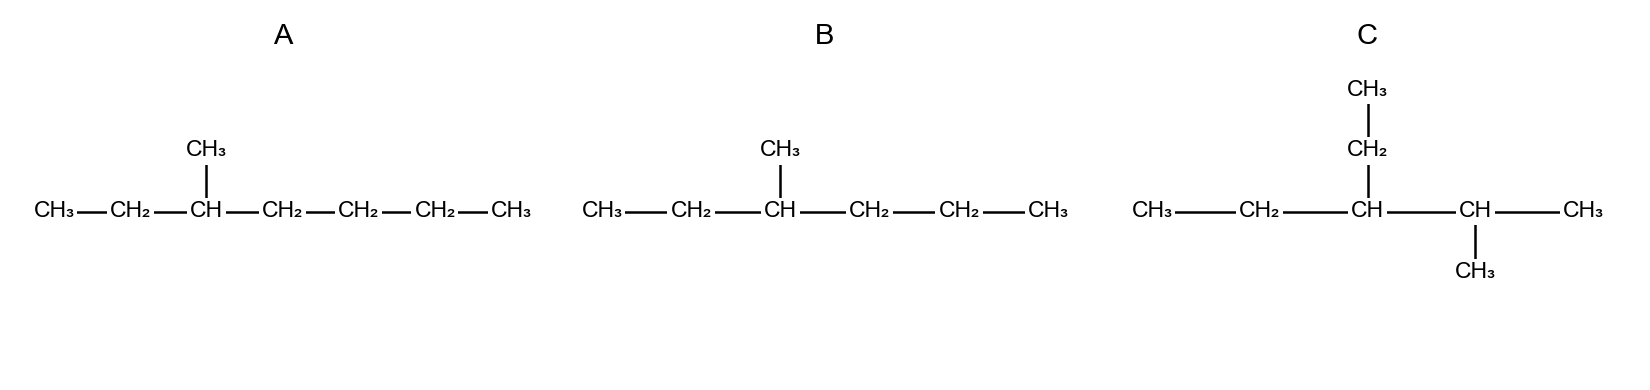
\includegraphics[width=0.86\linewidth]{rasmlar/gen/is_267791.png}\end{center}
Qaysi juftlik o`zaro izomerlar hisoblanadi?

\noindent A)~\textsl{A va B} \hfill B)~\textsl{B va C} \hfill C)~\textsl{A, B va C} \hfill D)~\textsl{A va C}\par
\vspace{4pt}
\noindent\textbf{27.} Uglevodlar haqida qaysi fikrlar to`g`ri? 1) Glyukoza gidrolizlanadi; 2) Kraxmal va selluloza bir xil M ga ega; 3) Selluloza $\beta$-glyukoza qoldiqlaridan iborat; 4) Saxaroza Feling suyuqligini qaytaradi

\noindent A)~\textsl{2, 3} \hfill B)~\textsl{3, 4} \hfill C)~\textsl{1, 3} \hfill D)~\textsl{3}\par
\vspace{4pt}
\noindent\textbf{28.} Aminlar, aminokislotalar va oqsillar haqida qaysi fikrlar to`g`ri? 1) Aminlar kuchsiz asoslar xossasini namoyon qiladi; 2) Aminokislotalar faqat kislotali xossaga ega; 3) Glitsin optik faol; 4) Dipeptidda 2 ta peptid bog` bor

\noindent A)~\textsl{1} \hfill B)~\textsl{3} \hfill C)~\textsl{3, 4} \hfill D)~\textsl{1, 2}\par
\vspace{4pt}
\noindent\textbf{29.} Izopren dan olingan polimerning polimerlanish darajasi 2500 bo`lsa, uning molyar \textbf{massasini (g/mol) aniqlang.}

\noindent A)~\textsl{85000} \hfill B)~\textsl{340000} \hfill C)~\textsl{2568} \hfill D)~\textsl{170000}\par
\vspace{4pt}
\end{multicols}
\noindent\textbf{30.} Uch probirkada (\textit{X}, \textit{Y}, \textit{Z}) AlCl\textsubscript{3}, MgCl\textsubscript{2}, KCl eritmalari bor (tartibsiz). Ularga NaOH ta'sir ettirildi. Kuzatuvlar jadvalda:
\begin{center}
\renewcommand{\arraystretch}{1.15}
\begin{tabular}{|c|c|c|}\hline
\textbf{Probirka} & \textbf{oz miqdor NaOH} & \textbf{mo`l miqdor NaOH} \\ \hline
\textit{X} & oq cho`kma & cho`kma mo`l ishqorda eriydi \\ \hline
\textit{Y} & oq cho`kma & cho`kma erimaydi \\ \hline
\textit{Z} & o`zgarish yo`q & --- \\ \hline
\end{tabular}
\end{center}
\textit{X}, \textit{Y}, \textit{Z} probirkalardagi \textbf{moddalarni aniqlang.}
\noindent A)~\textsl{\textit{X} -- KCl, \textit{Y} -- AlCl\textsubscript{3}, \textit{Z} -- MgCl\textsubscript{2}}\par
\noindent B)~\textsl{\textit{X} -- AlCl\textsubscript{3}, \textit{Y} -- MgCl\textsubscript{2}, \textit{Z} -- KCl}\par
\noindent C)~\textsl{\textit{X} -- KCl, \textit{Y} -- MgCl\textsubscript{2}, \textit{Z} -- AlCl\textsubscript{3}}\par
\noindent D)~\textsl{\textit{X} -- MgCl\textsubscript{2}, \textit{Y} -- KCl, \textit{Z} -- AlCl\textsubscript{3}}\par
\vspace{4pt}
\begin{multicols}{2}
\noindent\textbf{31.} Laboratoriyada olingan vodorod qanday usulda yig`iladi?
\noindent A)~\textsl{havoni siqib chiqarish (idish og`zi yuqoriga)}\par
\noindent B)~\textsl{suvni siqib chiqarish usulida yig`iladi}\par
\noindent C)~\textsl{H\textsubscript{2} suvni siqib chiqarish usulida yig`iladi}\par
\noindent D)~\textsl{havoni siqib chiqarish (idish og`zi pastga)}\par
\vspace{4pt}
\noindent\textbf{32.} Rasmda aralashmani ajratish usuli ko`rsatilgan. Bu \textbf{usulni toping.}
\begin{center}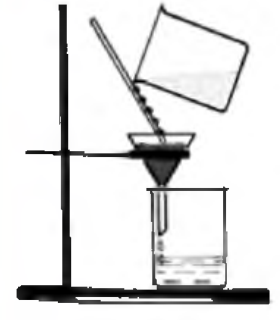
\includegraphics[width=0.86\linewidth]{rasmlar/darslik/d_filtr.png}\end{center}
\noindent A)~\textsl{distillash}\par
\noindent B)~\textsl{filtrlash}\par
\noindent C)~\textsl{magnit yordamida ajratish}\par
\noindent D)~\textsl{bug`latish   ---}\par
\vspace{4pt}
\end{multicols}
\medskip
\noindent\setlength{\fboxsep}{0pt}\fbox{\begin{tabular}{p{0.74\linewidth}|p{0.2\linewidth}}
\parbox[t]{0.72\linewidth}{\vspace{3pt}\textbf{Topshiriqlar (33--35) va javob variant (A--F)larini o`zaro to`g`ri moslashtiring.} Alyuminiy va magniy (Al va Mg) dan iborat 9 g qotishma mo`l HCl eritmasida eritilganda 10,08 l (n.sh.) gaz ajraldi.
\vspace{3pt}} & \parbox[t]{0.19\linewidth}{\vspace{3pt}A~\textsl{60}\\[3pt]
B~\textsl{246,38}\\[3pt]
C~\textsl{40,95}\\[3pt]
D~\textsl{131,4}\\[3pt]
E~\textsl{164,25}\\[3pt]
F~\textsl{61,43}}\\ \hline
\parbox[t]{0.72\linewidth}{\vspace{2pt}\textbf{33. Qotishmadagi Al massa ulushini (\%) aniqlang.}\vspace{2pt}} & \\ \hline
\parbox[t]{0.72\linewidth}{\vspace{2pt}\textbf{34. Reaksiya uchun sarflangan 20\% li HCl massasini (g) aniqlang.}\vspace{2pt}} & \\ \hline
\parbox[t]{0.72\linewidth}{\vspace{2pt}\textbf{35. Eritmadagi tuzlarning umumiy massasini (g) aniqlang.}\vspace{2pt}} & 
\end{tabular}}
\par\bigskip
\noindent\textbf{36.} Zn + HNO\textsubscript{3} $\to$ Zn(NO\textsubscript{3})\textsubscript{2} + NH\textsubscript{4}NO\textsubscript{3} + H\textsubscript{2}O reaksiya tenglamasini tenglang va barcha koeffitsiyentlar \textbf{yig`indisini aniqlang.}
\javob
\noindent\textbf{37.} 17 g H\textsubscript{2}O\textsubscript{2} reaksiyaga kirishdi (2H\textsubscript{2}O\textsubscript{2} $\to$ 2H\textsubscript{2}O + O\textsubscript{2}). Ajralgan O\textsubscript{2} \textbf{hajmini (l, n.sh.) hisoblang.}
\javob
\noindent\textbf{38.} Alyuminiy va mis dan iborat 9,1 g aralashma mo`l NaOH eritmasida eritildi. Ajralgan gazning \textbf{hajmini (l, n.sh.) aniqlang} (mis ishqor bilan reaksiyaga kirishmaydi).
\javob
\noindent\textbf{39.} 7,4 g propion kislota ni neytrallash uchun 10\% li NaOH eritmasidan necha gramm kerak?
\javob
\noindent\textbf{40.} Propilen dan olingan polimerning polimerlanish darajasi 100 bo`lsa, uning molyar \textbf{massasini (g/mol) aniqlang.}
\javob
\par\bigskip\begin{center}\textbf{\fontsize{13}{15}\selectfont YOZMA ISH}\end{center}
\noindent\textbf{41.} \textbf{Topshiriqni bajarish jarayonida barcha reaksiya tenglamalarini yozing. Miqdoriy va arifmetik hisoblashlarni (unga asos bo`lgan usul yoki formulani ko`rsatgan holda) uzviy ketma-ketlikda bajaring.}\par\smallskip
37,25 g KCl 300 g suvda eritildi. Hosil bo`lgan eritma inert elektrodlar yordamida 20 A tok kuchi bilan 965 s davomida elektroliz qilindi.\par
\noindent 1)Elektroliz tenglamasini yozing. Katodda va anodda ajralgan gazlarning hajmini (l, n.sh.) hisoblang (F = 96500 C/mol).\par
\noindent 2)Elektroliz qilingan KCl ning massasini (g) toping. Elektroliz davomida o`tgan zaryadni (C) ham hisoblang.\par
\noindent 3)Elektroliz tugagach eritmadagi KOH va qolgan KCl ning massa ulushlarini (\%) aniqlang.\par
\noindent 4)Anodda ajralgan gaz mo`l KI eritmasidan o`tkazildi. Ajralgan yodning massasini (g) hisoblang (reaksiya tenglamasini yozing). Neytrallash uchun sarflangan HCl miqdorini (mol) ham toping.\par
\noindent 5)Elektroliz tugagan eritmani to`liq neytrallash uchun 10\% li HCl eritmasidan necha gramm kerak? Elektroliz tugagan eritmadan mo`l CO\textsubscript{2} o`tkazilganda hosil bo`ladigan o`rta tuz (karbonat) massasini (g) ham hisoblang.\par
\diqqat{Mazkur topshiriq kengaytirilgan javobni talab etib, uning yechilish usuli va shu usul asosidagi barcha hisoblash amallari javoblar varaqasida aks etishi lozim.}
\noindent\textbf{42.} Quyidagi o`zgarishlar zanjirida \textit{X}, \textit{Y}, \textit{Z} noma'lum organik moddalar:\par
\[\setlength{\fboxsep}{0pt}\text{CH\textsubscript{3}COOC\textsubscript{2}H\textsubscript{5}}\xrightarrow{\text{NaOH}}\text{\textit{X}}\xrightarrow{\text{NaOH (suyuqlanma), t\textdegree{}}}\text{\textit{Y}}\xrightarrow{\text{Cl\textsubscript{2}, yorug`lik}}\text{\textit{Z}}\xrightarrow{\text{Na}}\text{C\textsubscript{2}H\textsubscript{6}}\]
\noindent 1)CH\textsubscript{3}COOC\textsubscript{2}H\textsubscript{5} $\to$ \textit{X} : reaksiya tenglamasini yozing; hosil bo`lgan moddani nomlang.\par
\noindent 2)\textit{X} $\to$ \textit{Y} : reaksiya tenglamasini yozing; hosil bo`lgan moddani nomlang.\par
\noindent 3)\textit{Y} $\to$ \textit{Z} : reaksiya tenglamasini yozing; hosil bo`lgan moddani nomlang.\par
\noindent 4)\textit{Z} $\to$ C\textsubscript{2}H\textsubscript{6} : reaksiya tenglamasini yozing; hosil bo`lgan moddani nomlang.\par
\diqqat{Mazkur topshiriq kengaytirilgan javobni talab etib, uning yechilish usuli va shu usul asosidagi barcha hisoblash amallari javoblar varaqasida aks etishi lozim.}
\noindent\textbf{43.} \textbf{Topshiriqni bajarish jarayonida barcha reaksiya tenglamalarini yozing. Miqdoriy va arifmetik hisoblashlarni (unga asos bo`lgan usul yoki formulani ko`rsatgan holda) uzviy ketma-ketlikda bajaring.}\par\smallskip
89,6 l (n.sh.) ammiak katalizator ishtirokida kislorodda oksidlandi (4NH\textsubscript{3} + 5O\textsubscript{2} $\to$ 4NO + 6H\textsubscript{2}O, unum 80\%). Hosil bo`lgan NO ni nitrat kislotagacha qayta ishlash unumi 80\%.\par
\noindent 1)Hosil bo`lgan NO hajmini (l, n.sh.) hisoblang. Hosil bo`lgan NO ning massasini (g) ham toping.\par
\noindent 2)Nitrat kislota ishlab chiqarishning keyingi bosqichlari tenglamalarini yozing va olingan HNO\textsubscript{3} massasini (g) toping.\par
\noindent 3)Hosil bo`lgan HNO\textsubscript{3} ni to`liq neytrallash uchun zarur ammiak hajmini (l, n.sh.) aniqlang (NH\textsubscript{3} + HNO\textsubscript{3} $\to$ NH\textsubscript{4}NO\textsubscript{3}).\par
\noindent 4)Hosil bo`lgan ammoniy nitrat massasini (g) hisoblang va azotning massa ulushini (\%) toping.\par
\noindent 5)Olingan HNO\textsubscript{3} dan 63\% li eritma necha gramm tayyorlanadi?\par
\diqqat{Mazkur topshiriq kengaytirilgan javobni talab etib, uning yechilish usuli va shu usul asosidagi barcha hisoblash amallari javoblar varaqasida aks etishi lozim.}
\newpage
\noindent\textbf{\fontsize{13}{15}\selectfont Nazorat testi}\ \textit{$\cdot$ 20-variant}\hfill \textbf{Javoblar kaliti}\par\smallskip\hrule\smallskip
\textit{Faqat o`qituvchi uchun.}\par\medskip
\noindent\textbf{1--32-savollar}\par\smallskip
\noindent\begin{tabular}{|c|c|c|c|c|c|c|c|c|c|c|c|c|c|c|c|}\hline
\textbf{1} & \textbf{2} & \textbf{3} & \textbf{4} & \textbf{5} & \textbf{6} & \textbf{7} & \textbf{8} & \textbf{9} & \textbf{10} & \textbf{11} & \textbf{12} & \textbf{13} & \textbf{14} & \textbf{15} & \textbf{16}\\\hline
\textsl{A} & \textsl{A} & \textsl{A} & \textsl{B} & \textsl{B} & \textsl{C} & \textsl{B} & \textsl{A} & \textsl{D} & \textsl{B} & \textsl{A} & \textsl{C} & \textsl{D} & \textsl{C} & \textsl{C} & \textsl{B}\\\hline
\textbf{17} & \textbf{18} & \textbf{19} & \textbf{20} & \textbf{21} & \textbf{22} & \textbf{23} & \textbf{24} & \textbf{25} & \textbf{26} & \textbf{27} & \textbf{28} & \textbf{29} & \textbf{30} & \textbf{31} & \textbf{32}\\\hline
\textsl{C} & \textsl{A} & \textsl{D} & \textsl{A} & \textsl{C} & \textsl{D} & \textsl{B} & \textsl{D} & \textsl{C} & \textsl{D} & \textsl{D} & \textsl{A} & \textsl{D} & \textsl{B} & \textsl{C} & \textsl{B}\\\hline
\end{tabular}\par\medskip
\noindent\textbf{33--35-savollar}\par\smallskip
\noindent\begin{tabular}{|c|c|c|}\hline \textbf{No} & \textbf{Javob} & \textbf{Qiymat}\\\hline
33 & \textsl{A} & 60\\\hline
34 & \textsl{E} & 164,25\\\hline
35 & \textsl{C} & 40,95\\\hline
\end{tabular}\par\medskip
\noindent\textbf{36--40-savollar}\par\smallskip
\noindent\begin{tabular}{|c|c|}\hline \textbf{No} & \textbf{To`g`ri javob}\\\hline
36 & 22\\\hline
37 & 5,6\\\hline
38 & 3,36\\\hline
39 & 40\\\hline
40 & 4200\\\hline
\end{tabular}\par\medskip
\noindent\textbf{41--43-topshiriqlar: qisqa yechim}\par\smallskip
\noindent\textbf{41-topshiriq.}\par
\noindent 1) 2KCl + 2H\textsubscript{2}O $\to$ 2KOH + H\textsubscript{2}$\uparrow$ + Cl\textsubscript{2}$\uparrow$. n(e\textsuperscript{$-$}) = It/F = 20$\cdot$965/96500 = 0,2 mol; n(H\textsubscript{2}) = n(Cl\textsubscript{2}) = 0,1 mol $\to$ \textit{V} = \textbf{2,24 l} (har biri)\par
\noindent 2) n(KCl) = n(e\textsuperscript{$-$})/1 = 0,2 mol; m = 0,2$\cdot$74,5 = \textbf{14,9 g}; Q = 20$\cdot$965 = \textbf{19300 C}\par
\noindent 3) m(eritma) = 37,25 + 300 $-$ 0,2 (H\textsubscript{2}) $-$ 7,1 (Cl\textsubscript{2}) = 329,95 g; $\omega$(KOH) = 11,2/329,95 = \textbf{3,39\%}; $\omega$(KCl) = 22,35/329,95 = \textbf{6,77\%}\par
\noindent 4) Cl\textsubscript{2} + 2KI $\to$ 2KCl + I\textsubscript{2}: n(I\textsubscript{2}) = 0,1 mol $\to$ m = \textbf{25,4 g}; n(HCl) = 0,2 mol\par
\noindent 5) KOH + 1 HCl $\to$ ...: n(HCl) = 0,2 mol = 7,3 g; 10\% li eritma: 7,3/0,1 = \textbf{73 g}; CO\textsubscript{2} + 2KOH $\to$ karbonat: n = 0,1 mol $\to$ \textbf{13,8 g}\par
\noindent Jami: M 15 + A 10 = 25 ball.\par
\noindent\textbf{42-topshiriq.}\par
\noindent 1) CH\textsubscript{3}COOC\textsubscript{2}H\textsubscript{5} + NaOH $\to$ CH\textsubscript{3}COONa (natriy atsetat)\par
\noindent 2) CH\textsubscript{3}COONa + NaOH (suyuqlanma), t\textdegree{} $\to$ CH\textsubscript{4} (metan)\par
\noindent 3) CH\textsubscript{4} + Cl\textsubscript{2}, yorug`lik $\to$ CH\textsubscript{3}Cl (xlormetan)\par
\noindent 4) CH\textsubscript{3}Cl + Na $\to$ C\textsubscript{2}H\textsubscript{6} (etan)\par
\noindent Jami 25 ball.\par
\noindent\textbf{43-topshiriq.}\par
\noindent 1) n(NH\textsubscript{3}) = 4 mol; n(NO) = 4$\cdot$0,8 = 3,2 mol $\to$ \textbf{71,68 l}; m(NO) = 3,2$\cdot$30 = \textbf{96 g}\par
\noindent 2) 2NO + O\textsubscript{2} $\to$ 2NO\textsubscript{2}; 4NO\textsubscript{2} + O\textsubscript{2} + 2H\textsubscript{2}O $\to$ 4HNO\textsubscript{3}: n(HNO\textsubscript{3}) = 2,56 mol $\to$ \textbf{161,28 g}\par
\noindent 3) NH\textsubscript{3} : HNO\textsubscript{3} = 1 : 1 $\to$ \textbf{57,34 l}\par
\noindent 4) NH\textsubscript{4}NO\textsubscript{3}: 2,56 mol $\cdot$ 80 = \textbf{204,8 g}; $\omega$(N) = 28/80 = \textbf{35\%}\par
\noindent 5) m(eritma) = 161,28/0,63 = \textbf{256 g}\par
\noindent Jami: M 15 + A 10 = 25 ball.\par
\par\bigskip\noindent\textbf{Mavzular taqsimoti}\par\smallskip
{\small\noindent\begin{longtable}{|c|p{7.2cm}|p{5.4cm}|c|}\hline \textbf{No} & \textbf{Mavzu} & \textbf{Tekshiriladigan ko`nikma} & \textbf{Ball}\\\hline
1 & 11-sinf (Mendeleyev--Klapeyron) & Hisoblash va masala yechish & 1\\\hline
2 & 9-sinf (gidroliz); Tirkashev IV bob & Bilim va tushunish & 1\\\hline
3 & 7-sinf (jism va modda) & Bilim va tushunish & 1\\\hline
4 & 8-sinf (kimyoviy bog`lanish turlari, jadval) & Jadval tahlili & 1\\\hline
5 & Tirkashev IV bob (kuchli elektrolitlar) & Hisoblash va masala yechish & 1\\\hline
6 & Tirkashev VI bob; 11-sinf (muvozanat) & Hisoblash va masala yechish & 1\\\hline
7 & 11-sinf (gaz aralashmalar) & Hisoblash va masala yechish & 1\\\hline
8 & Tirkashev I bob; 8-sinf (elektron konfiguratsiya) & Bilim va tushunish & 1\\\hline
9 & Tirkashev III bob (eruvchanlik, grafik) & Grafik tahlili & 1\\\hline
10 & Tirkashev III bob (eritmalar, jadval) & Jadval tahlili & 1\\\hline
11 & 11-sinf (Mendeleyev--Klapeyron) & Hisoblash va masala yechish & 1\\\hline
12 & Tirkashev VI bob (Le-Shatelye) & Bilim va tushunish & 1\\\hline
13 & 11-sinf 8-bob; Tirkashev \textit{V} bob (elektroliz) & Bilim va tushunish & 1\\\hline
14 & 9-sinf (ishqoriy metallar); Tashev & Bilim va tushunish & 1\\\hline
15 & 9-sinf (alyuminiy) & Hisoblash va masala yechish & 1\\\hline
16 & 9-sinf; Tashev (Fe, Cu, Zn, Cr) & Bilim va tushunish & 1\\\hline
17 & 9-sinf; Tirkashev (suv qattiqligi, hisob) & Hisoblash va masala yechish & 1\\\hline
18 & 9-sinf; Tirkashev (oksid/asos/kislota/tuz, hisob) & Hisoblash va masala yechish & 1\\\hline
19 & 9-sinf; Tirkashev (genetik zanjir/reaksiya turlari, hisob) & Hisoblash va masala yechish & 1\\\hline
20 & 10-sinf (alkan, hisob) & Hisoblash va masala yechish & 1\\\hline
21 & 10-sinf (nomenklatura \S{}6, \S{}11, \S{}20, \S{}24--26) & Bilim va tushunish & 1\\\hline
22 & 10-sinf (mavzuga oid paragraflar); Abdusamatov & Bilim va tushunish & 1\\\hline
23 & 10-sinf (ikki bosqichli hisob) & Hisoblash va masala yechish & 1\\\hline
24 & 10-sinf (ikki bosqichli hisob) & Hisoblash va masala yechish & 1\\\hline
25 & 10-sinf \S{}6, \S{}12, \S{}20, \S{}28 (izomeriya) & Bilim va tushunish & 1\\\hline
26 & 10-sinf (izomeriya) & Rasm bo`yicha tahlil & 1\\\hline
27 & 10-sinf (mavzuga oid paragraflar); Abdusamatov & Bilim va tushunish & 1\\\hline
28 & 10-sinf (mavzuga oid paragraflar); Abdusamatov & Bilim va tushunish & 1\\\hline
29 & 10-sinf \S{}35 (YuMB) & Hisoblash va masala yechish & 1\\\hline
30 & 7--10-sinf va Tashev (laboratoriya ishlari, sifat reaksiyalar) & Jadval tahlili & 1\\\hline
31 & 9--10-sinf (gazlarni yig`ish) & Bilim va tushunish & 1\\\hline
32 & 7-sinf (11-rasm) & Rasm bo`yicha tahlil & 1\\\hline
33--35 & Aralash masala (moslashtirish) & Ko`p bosqichli hisob & 3\\\hline
36--40 & Qisqa javobli masalalar & Hisoblash & 5\\\hline
41--43 & Yozma ish & Usul va hisob (M, A) & 75\\\hline
\end{longtable}}
\end{document}
